\documentclass[11pt ,twosided]{article}
%\usepackage{graphicx}
%\usepackage{algorithm}
%\usepackage{algorithmic}
\usepackage[margin=0.9in]{geometry}

\title{Enhancement to eXpOS Operating System and eXpFS File System}

\author{ Kruthika Suresh Ved     B110300CS\\  Sikha V Manoj     B110572CS\\  Sonia V Mathew    B110495CS\\ Guided by: Dr.K.Muralikrishnan}

\usepackage{epsfig}
\begin{document}
\maketitle
	

\abstract{} 

Project eXpOS or experimental Operating System is a educational platform to develop an operating system. It is an instructional tool for students to learn and implement OS data structures and functionalities on a simulated machine called XSM (eXperimental String Machine).The OS is programmed using a custom language known as SPL (System Programmer's Language) and application programs, which run on the OS, are programmed using eXpL (Experimental Programmer's Language).


\section{Problem Definition}

This project aims to extend eXpOS with features like Shared Memory Model, Inter\-Process Communication, Synchronization and Directory Structure.
\section{eXpOS Specification}

eXpOS has a very simple specification that allows a junior undergraduate computer science student to implement it in a few months, subject to availability of adequate hardware and programming platform support. This OS specification is prepared in a manner independent of programming language and target machine.
\subsection{eXperimental File System (eXpFS)}

eXpOS uses eXpFS (eXperimental File System) which contains files organized into a single directory called the root. There are three types of eXpFS files: the root, data files and executable files. The root is also treated conceptually as a file.
\subsubsection{Root}

The root file has name \textbf {root} and contains information about the files stored in the file system. For each file stored in eXpFS, the root stores three words of information: file-name, file-size and file-type. This triple is called the root entry for the file. The first root entry is for the root itself.  
\subsubsection{Data File}

A data file is a sequence of words. eXpFS expects the Operating System to display data files with an extension .dat.   eXpFS treats this as a default file type, hence the application programs do not have to specify the extension .dat at the time of file creation.  
The operations allowed in data files are Create, Delete, Open, Close, FLock, FUnlock, Read, Write, Seek.
\subsubsection{Executable File}

Executable files are essentially program files that must be loaded and run by the operating system. The executable file format recognized by eXpOS is called the Experimental executable file (XEXE) format. In this format, an executable file is divided into two sections - Header and Code (In this implementation of eXpOS, static data is stored in stack pages).
\subsection{Process Model}

A program under execution is called a process. The eXpOS associates a virtual (memory) address space for each process. The eXpOS logically partitions the address space into four regions: library, code, stack and heap. These regions are mapped into physical memory using hardware mechanisms like paging/segmentation.
%\begin{figure}[ht]
%\centering
%\includegraphics[scale=0.75]{P_Model.png}
%\caption{\footnotesize Process Model in eXpOS}
%\label{fig_1}
%\end{figure}
\subsection{Inter\-Process Communication}

eXpOS assumes a single processor multi programming environment. It allows processes to communicate with each other using mechanisms like semaphores and Wait\-Signal system calls.
eXpOS provides (binary) semaphores to allow application programs to handle the critical section problem. eXpOS provides system calls like Semget, SemLock, SemUnlock, Semrelease for working with semaphores.
\subsection{Shared Memory Model}

Shared memory is an efficient means of sharing data between programs. In eXpOS, this sharing is done between the parent process and child processes (or any child process in the hierarchy) through heap. It is the responsibility of the programmer to ensure exclusive access to the shared resources for each process, to avoid data inconsistency. eXpOS helps programmer to realize data consistency with the help of semaphores. 
\subsection{System Calls}

Application programmers interact with the Operating System using the system calls. When a process invokes a system call, the process is interrupted and control goes to the corresponding interrupt service routine of the kernel, resulting in a switch from user mode to kernel mode. Once the system call is carried out, the control goes back to the application program, with a switch back to the user mode.\\
The following system calls are present in the system: 
\begin{itemize}
\item File System Calls : Create, Delete, Open, Close, Read, Write, Seek
\item Process System Calls : Fork, Exec, Exit, Getpid, Getppid, Shutdown
\item System calls for access control and Synchronization: Wait, Signal, FLock, FUnLock, Semget, Semrelease, SemLock, SemUnLock.
\end{itemize}

\subsection{Pre-Emptive Scheduling}

In Pre-Emptive Scheduling, process can be paused before its time slice is over. This usually happens when a resource that the process requires is not available at the present. The process puts itself to sleep and another process is scheduled for execution.
\subsection{Asynchronous disk operations}

To minimize processor cycles spent on disk operations, disk operations are made asynchronous. This means that while a disk operation is being carried out, other processes which do not require the disk can be executed.
\section{Design of eXpOS}
\subsection{Data Structures}

The OS data structures store information about processes, files and semaphores. eXpOS data structures can be divided into - Disk Data structures and Memory (in-core) data structures. A copy of Disk Data Structures will be kept in the memory while the system is running.
\subsection{Disk Data Structures}
\subsubsection{Inode Table}

Inode Table is the record of the files stored in the disk. The entry of an Inode table has the following format:
\begin{figure}[ht]
\centering
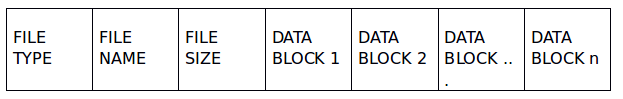
\includegraphics[scale=0.60]{Inode_table.png}
\caption{\footnotesize Structure of the Inode Table}
\label{fig_1}
\end{figure}
\subsubsection{Disk Free List}

For each block in the disk there is an entry in the Disk Free List which contains a value of either 0 or 1 indicating whether the corresponding block in the disk is free or used.
\subsection{Memory Data Structures}
\subsubsection{Process Table}

The Process Table contains an entry for each process.  Each entry contains several fields that stores all the information pertaining to a single process. The maximum number of entries is equal to maximum number of processes allowed to exist at a single point of time in eXpOS.
\begin{figure}[ht]
\centering
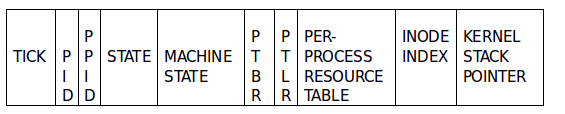
\includegraphics[scale=0.60]{Process_table.png}
\caption{\footnotesize Structure of the Process Table}
\label{fig_2}
\end{figure}
\\

The first entry Tick keeps track of how long the process was in memory.

The second column is PID or Process ID which is a number that is unique to each process.

The third column gives the process descriptor of the parent process or the PPID.

Next column, State , consists of a two tuple that describes the current state of the process.

The fifth column is the pointer to a structure that gives the Machine State when the process was last executed.  This part is machine dependent. 

The next two columns are regarding the page table of the process. The first one (PTBR or Page Table Base Register) stores the starting address of the page table of a process while the next one (PTLR or Page Table Length Register) stores the number of entries in the page table of a process and determines the size of the virtual address space of the process.

The next column is a pointer to a table, the Per-Process Resource Table that contains information about the files opened by the process as well as semaphores used by the process.

Inode Index is a reference to the Inode entry of the executable file. It could be used to access the code pages of the process.

Each process has its own kernel stack. The pointer to the kernel stack is given in the Kernel Stack Pointer column. A process uses its kernel stack to save the return address when it voluntarily schedule out itself inside a blocking system call. 
\subsubsection{Per-Process Resource Table}
This table stores information about the resources (files/semaphores) acquired by the process. For every file opened by the process, it stores the index of the File Table entry for the file, and the LSEEK position of the open instance of a file. The LSEEK position indicates the location in the file where the next read/write operation occurs. Similarly, for every semaphore used by the process, the Per-Process resource table stores the index of Semaphore Table entry. 
\begin{figure}[ht]
\centering
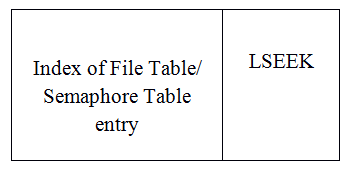
\includegraphics[scale=0.60]{PerProcessResource_table.png}
\caption{\footnotesize Structure of the Per-Process Resource Table}
\label{fig_3}
\end{figure}

\subsubsection{Page Table}
The Page Table contains information relating to the actual location of the pages of the process in the memory. The page table contains physical page numbers corresponding to logical pages in the virtual address space of the process. Each entry has a reference bit and a valid bit. Reference bit indicates whether the page is referenced by the process or not. Valid bit indicates whether the page is present in memory or not.
\begin{figure}[ht]
\centering
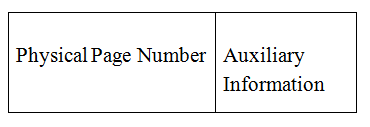
\includegraphics[scale=0.60]{Page_table.png}
\caption{\footnotesize Structure of Page Table}
\label{fig_4}
\end{figure}
\subsubsection{File Table}

File Table has information about all the files that are currently open.  The Open system call creates an entry in the File table when a process opens a file that is not opened by any process in execution. If the file is opened again by some other process (or the same process), the Open system call updates the same file table entry.
\begin{figure}[ht]
\centering
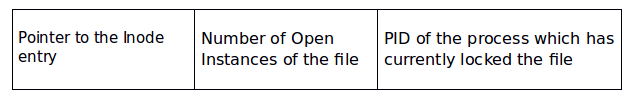
\includegraphics[scale=0.60]{File_table.png}
\caption{\footnotesize Structure of the File Table}
\label{fig_5}
\end{figure}
\subsubsection{Semaphore Table}

Semaphore Table contains details about all the semaphores used by the processes. For every semaphore opened by a process, there is an entry in the Per-Process resource table,  and this entry points to a corresponding entry in the semaphore table.
\begin{figure}[ht]
\centering
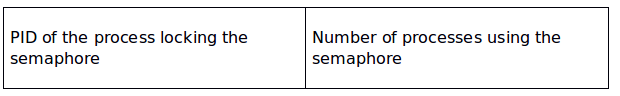
\includegraphics[scale=0.60]{Semaphore_Table.png}
\caption{\footnotesize Structure of the Semaphore Table}
\label{fig_6}
\end{figure}
\subsubsection{Disk Status Table}

eXpOS makes use of Disk Status Table to keep track of load and store operations. It consists of a bit to determine the type of disk operation (load/store), the numbers of page and block involved in the disk operation and the process identifier of the process which initiated disk transfer.
\begin{figure}[ht]
\centering
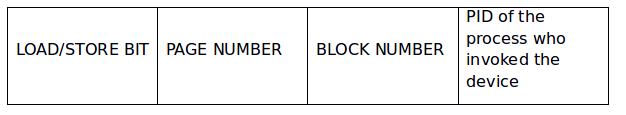
\includegraphics[scale=0.60]{Disk_Status.png}
\caption{\footnotesize Structure of the Disk Status Table}
\label{fig_7}
\end{figure}
\subsubsection{Buffer Table}

To minimize the number of load and store operations, eXpOS provides a buffer cache in memory which would temporarily store disk blocks. Each disk block is mapped to a unique buffer. The disk blocks will be stored back to the disk when some other blocks replace it. Only modified blocks are written back to disk.
Buffer Table keeps the information about disk blocks present in the buffer.
\begin{figure}[ht]
\centering
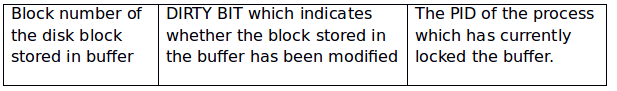
\includegraphics[scale=0.60]{Buffer_table.png}
\caption{\footnotesize Structure of the Buffer Table}
\label{fig_8}
\end{figure}
\subsubsection{System Status Table}

System Status Table keeps the information about number of free pages in memory (MEM\_FREE\_COUNT), number of processes waiting for memory pages (WAIT\_MEM\_COUNT), and also the number of processes which have been swapped out to the disk (SWAPPED\_COUNT).
\subsubsection{Memory Free List}

The Memory free list is a data structure used for keeping track of used and unused pages in the memory. Each entry of the free list contains a value of either 0, indicating whether the corresponding page in the memory is free or a number ($>$0), indicating the number of processes that share the page.
\subsection{Algorithms}
\subsubsection{File System Calls}
%%%%% Create System Call %%%%%%%%%%%%%%%
\textbf{1. Create System Call}
\vspace{3mm}\\
The Create operation takes as input a filename and creates an empty file by that name. If a root entry for the file already exists, then the system call returns 0 (success). Otherwise, it creates a root entry for the file name, sets the file type to DATA and file size to 0. Note that the file name must be a character string and must not be “root”. 
\begin{description}
\item[Arguments]: Filename
\item[Return Value]: 0 (Success) or -1 (No Space for file)
\end{description}
\iffalse
\vspace{3mm}
\begin{algorithm}
\caption{Create system call}
\begin{algorithmic}
\IF{file is present in Inode Table}
    \RETURN 0 
\ENDIF    
\IF{no free entry in Inode Table}
    \RETURN -1 
\ELSE
    \STATE Store index of free entry in \textit{InodeIndex}
\ENDIF   
\STATE In the Inode Table entry corresponding to \textit{InodeIndex}, set file name to Filename, file size to 0 and file type to “DATA ”.
\STATE In the root file entry corresponding to \textit{InodeIndex}, set file name to Filename, file size to 0 and file type to “DATA ”.
\STATE Increment the root file size
\RETURN 0 
\end{algorithmic}
\end{algorithm}
\fi
\textbf{2. Delete System Call}
\vspace{3mm}\\
Delete removes the file from the file system and removes its root entry. A file that is currently opened by any application cannot be deleted. Root file also cannot be deleted.
\begin{description}
	\item[Arguments]: Filename
	\item[Return Value]: 0 (Success) or -1 (File not found) or -2 (File is open)
\end{description} 
\iffalse
\begin{algorithm}
\caption{Delete system call}
\begin{algorithmic}
\IF{file is not present in Inode table}
    \RETURN -1
\ELSE
    \STATE Store index of file in \textit{InodeIndex}
\ENDIF    
\IF{file is open}
    \RETURN -2
\ENDIF
\STATE Free all the blocks allocated to the file
\STATE Invalidate the Inode Table entry corresponding to \textit{InodeIndex}
\STATE Remove root file entry corresponding to \textit{InodeIndex}
\STATE Decrement the file size of root file
\RETURN 0 
\end{algorithmic}
\end{algorithm}
\fi
\textbf{3. Open System Call}
\vspace{3mm}\\
For a process to read/write a file, it must first open the file. Only data and root files can be opened. The Open operation returns a file descriptor. An application can open the same file several times and each time, a different descriptor will be returned by the Open operation. The file descriptor must be passed as argument to other file system calls, to identify the open instance of the file.
\vspace{2mm}\\
The OS associates a file pointer with every open instance of a file. The file pointer indicates the current location of file access (read/write). The Open system call sets the file pointer to 0 (beginning of the file).
\vspace{2mm}
\begin{description}
	\item[Arguments]: Filename
	\item[Return Value]: File Descriptor (Success) or -1 (File not found) or -2 (Process has reached its limit of resources) or -3 ( 	System has reached its limit of open files)
\end{description} 
\iffalse
\begin{algorithm}
\caption{Open system call}
\begin{algorithmic}
\IF{file is not found in Inode Table}
    \RETURN -1
\ENDIF
\IF{file type is not DATA or ROOT}
    \RETURN -1
\ENDIF
\IF{no free entry in Per-Process Resource table}
    \RETURN -2
\ELSE
    \STATE Store index of free entry in \textit{PerProcessIndex}
\ENDIF    
\IF{file is already open}
    \STATE Store index of file table entry in \textit{FTIndex}
\ELSE
    \IF{no free entry in File Table}
        \RETURN -2
    \ELSE 
        \STATE Store index of free entry in \textit{FTIndex}
    \ENDIF
\ENDIF
\STATE In entry corresponding to \textit{PerProcessIndex}, set pointer to File Table as \textit{FTIndex} and LSEEK as 0
\STATE In entry corresponding to \textit{FTIndex}, set pointer to Inode Table as \textit{InodeIndex} 
\STATE Increment file open count
\STATE Set lock status to free
\RETURN \textit{PerProcessIndex} 
\end{algorithmic}
\end{algorithm}
\vspace{5mm}
\fi
\textbf{4. Close System Call}
\vspace{2mm}\\
 After all the operations are done, the user closes the file using the Close system call. The file descriptor ceases to be valid once the close system call is invoked. 
\begin{description}
	\item[Arguments]: File Descriptor
	\item[Return Value]: 0 (Success) or -1 (File Descriptor is invalid)
\end{description} 
\iffalse
\begin{algorithm}
\caption{Close system call}
\begin{algorithmic}
\IF{File Descriptor is not valid}
    \RETURN -1
\ENDIF
\IF{entry in Per-Process Resource table is not valid}
    \RETURN -1
\ELSE 
    \STATE Store the pointer to File Table in  \textit{FTIndex}
\ENDIF
\IF{file is locked by current process}
    \STATE Unlock the file
\ENDIF
\STATE Decrement file open count
\IF{file open count becomes zero }
    \STATE Invalidate the File Table entry
    \ENDIF
\STATE Invalidate Per-Process Table entry 
\RETURN 0
\end{algorithmic}
\end{algorithm}
\fi
\textbf{5. Read System Call}
\vspace{2mm}\\
The file descriptor is used to identify an open instance of the file. The Read operation reads one word from the position pointed by the file pointer and stores it into the buffer. After each read operation, the file pointer advances to the next word in the file. 
\begin{description}
	\item[Arguments]: File Descriptor and a Buffer (a String/Integer variable) into which a word is to be read from the file
	\item[Return Value]: 0 (Success) or -1 (File Descriptor is invalid) or -2 (File pointer has reached the end of file)
\end{description} 
\iffalse
\begin{algorithm}
\caption{Read system call}
\begin{algorithmic}
\IF{File Descriptor is not valid}
    \RETURN -1
\ENDIF
\IF{entry in Per-Process Resource table is not valid}
    \RETURN -1
\ELSE 
    \STATE Store the pointer to File Table in  \textit{FTIndex}
    \STATE Store LSEEK in \textit{lseek}
\ENDIF
\IF{file is locked}
    \IF{current process has not locked the file}
        \WHILE{file is locked}
            \STATE Put the current process to sleep
            \STATE Call scheduler
        \ENDWHILE
    \ENDIF
\ENDIF
\STATE Lock the file
\STATE Store pointer to Inode Table in  \textit{InodeIndex}
\IF{file pointer is at the end of the file}
    \RETURN -2
\ELSE 
    \STATE Store \textit{lseek}/block-size in \textit{BlockNum}
    \STATE Store \textit{lseek}\%block-size in \textit{Offset}
\ENDIF
\IF{buffer to which the block is mapped is locked}
    \IF{current process has not locked the buffer}
        \WHILE{buffer is locked}
            \STATE Put the process to sleep 
            \STATE Call scheduler
        \ENDWHILE
    \ENDIF
\ENDIF
\STATE Lock the buffer
\IF{buffer does not have required block}
    \IF{buffer contains a block and dirty bit is set}
        \STATE Store the block in buffer to disk
    \ENDIF
    \STATE Load the required block to the buffer
\ENDIF
\STATE Read the data and increment the file pointer
\STATE Unlock the buffer and wake all processes waiting for the buffer
\STATE Unlock the file and wake all processes waiting for the file
\RETURN 0
\end{algorithmic}
\end{algorithm}
\vspace{3mm}
\fi
\textbf{6. Write System Call}
\vspace{2mm}\\
The file descriptor is used to identify an open instance of the file. The Write operation writes the word stored in the buffer to the position pointed by the file pointer of the file. After each Write operation, the file pointer advances to the next word in the file.
\begin{description}
	\item[Arguments]:File Descriptor and a Word to be written
	\item[Return Value]: 0 (Success) or -1 (File Descriptor given is invalid) or -2 (No disk space)
\end{description} 
\iffalse
\begin{algorithm}
\caption{Write system call}
\begin{algorithmic}
\IF{File Descriptor is not valid}
    \RETURN -1
\ENDIF
\IF{entry in Per-Process Resource table is not valid}
    \RETURN -1
\ELSE 
    \STATE Store the pointer to File Table in \textit{FTIndex} and LSEEK in \textit{lseek}
\ENDIF
\IF{file is locked}
    \IF{current process has not locked the file}
        \WHILE{file is locked}
            \STATE Put the current process to sleep and call scheduler
        \ENDWHILE
    \ENDIF
\ENDIF
\STATE Lock the file
\STATE Store pointer to Inode Table in \textit{InodeIndex}
\STATE Store \textit{lseek}/block-size in \textit{BlockNum} and \textit{lseek}\%block-size in \textit{Offset}
\IF{entry in Inode Table corresponding to \textit{BlockNum} is invalid}
    \IF{no free block in disk}
        \RETURN -2
    \ELSE
        \STATE Allocate a free block to the file
        \STATE Increment file size in Inode Table and root file
    \ENDIF
\ENDIF
\IF{buffer to which the block is mapped is locked}
    \IF{current process has not locked the buffer}
        \WHILE{buffer is locked}
            \STATE Put the process to sleep and call scheduler
        \ENDWHILE
    \ENDIF
\ENDIF
\STATE Lock the buffer
\IF{buffer does not have required block}
    \IF{buffer contains a block and dirty bit is set}
        \STATE Store the block in buffer to disk
    \ENDIF
    \STATE Load the required block to the buffer
\ENDIF
\STATE Write the data and increment file pointer
\STATE Unlock the buffer and wake all processes waiting for the buffer
\STATE Unlock the file and wake all processes waiting for the file
\RETURN 0
\end{algorithmic}
\end{algorithm}
\vspace{3mm}
\fi
\textbf{7. Seek System Call}
\vspace{3mm}\\
The Seek operation allows the application program to change the value of the file pointer so that subsequent Read/Write is performed from a new position in the file. The new value of the file pointer is determined by adding the offset to the current value. (A negative Offset will move the pointer backwards). An Offset of 0 will reset the pointer to the beginning of the file. 
\begin{description}
	\item[Arguments]: File Descriptor and Offset
	\item[Return Value]: 0 (Success) or -1 (File Descriptor given is invalid) or -2 (Offset value moves the file pointer to a position outside the file)
\end{description} 
\iffalse
\begin{algorithm}
\caption{Seek system call}
\begin{algorithmic}
\IF{File Descriptor is not valid}
    \RETURN -1
\ENDIF
\IF{entry in Per-Process Resource table is not valid}
    \RETURN -1
\ELSE 
    \STATE Store the pointer to File Table in \textit{FTIndex}
    \STATE Store LSEEK in \textit{lseek}
\ENDIF
\IF{file is locked}
    \IF{current process has not locked the file}
        \WHILE{file is locked}
            \STATE Put the current process to sleep 
            \STATE Call scheduler
        \ENDWHILE
    \ENDIF
\ENDIF
\STATE Lock the file
\STATE Store pointer to Inode Table in \textit{InodeIndex}
\IF{new file pointer is not valid}
    \RETURN -2
\ENDIF
\IF{Offset is zero}
    \STATE Set LSEEK to beginning of file
\ELSE
    \STATE Set LSEEK to LSEEK$+$Offset
\ENDIF
\STATE Unlock the file and wake all processes waiting for the file
\RETURN 0
\end{algorithmic}
\end{algorithm}
\vspace{15mm}
\fi
\subsubsection{Process System Calls}
\textbf{1. Fork System Call}
\\
Replicates the process invoking the system call. The heap, code and library regions of the parent are shared by the child. A new stack is allocated to the child and the parent's stack is copied into the child's stack.
\\
When a process executes the Fork system call, the child process shares with the parent all the file and semaphore descriptors previously acquired by the parent. Semaphore/file descriptors acquired subsequent to the fork operation by either the child or the parent will be exclusive to the respective process and will not be shared.
\begin{description}
\item[Arguments]: None
\item[Return Value]: Process Identifier to the parent process and 0 to child process (Success) or -1 (Number of processes has reached its maximum, returned to parent)
\end{description} 
\iffalse
\begin{algorithm}
\caption{Fork system call}
\begin{algorithmic}
\IF{no free entry in process table}
    \RETURN -1
\ELSE
    \STATE Store index of free entry in \textit{ChildPID}
    \STATE Store pid of parent process in \textit{ParentPID}
\ENDIF
\STATE Set the PPID field of child process to \textit{ParentPID}
\STATE Count the number of stack pages of parent
\WHILE{equal number of free pages are not present in memory}
    \STATE Put the process to sleep
    \STATE Call scheduler
\ENDWHILE
\STATE Allocate one free page to the child for each stack page of the parent
\STATE Copy the parent's stack to child's stack
\STATE Copy the page table entries, except stack entries, of parent to the page table of child
\STATE Copy the parent's machine state and Per-Process resource table to the child
\STATE Copy the inode index from parent to child 
\STATE For every open file of the parent, increment the file open count
\STATE For every semaphore acquired by the parent, increment process count
\STATE Set state of child to ready
\RETURN 0 to the child process and \textit{ChildPID} to the parent process
\end{algorithmic}
\end{algorithm}
\vspace{22mm}
\textbf{Exec System Call}
\\
Exec destroys the present process and loads the executable file given as input into a new memory address space. A successful Exec operation results in the extinction of the invoking application and hence never returns to it. All open instances of file and semaphores of the parent process are closed. However, the newly created process will inherit the PID of the calling process.
\begin{description}
\item[Arguments]: Filename
\item[Return Value]: -1 (File not found or file is of invalid type)
\end{description} 
\begin{algorithm}
\caption{2. Exec system call}
\begin{algorithmic}
\IF{file not found in Inode Table}
    \RETURN -1
\ELSE
    \IF{file type is not EXEC}
        \RETURN -1
    \ELSE
        \STATE Store index of Inode Table entry in \textit{InodeIndex}
        \STATE Store the code block numbers of the file in \textit{Block1} and \textit{Block2}.
    \ENDIF
\ENDIF
\STATE In the page table of current process, set code page entries to \textit{Block1} and \textit{Block2}.
\STATE Set the auxiliary information of code pages to invalid and unreferenced.
\STATE Include the page numbers of shared library in the page table.
\STATE Invalidate the entry for heap pages
\STATE In the process table of current process, set the pointer to Inode Table as \textit{InodeIndex}
\STATE Close all files opened by the current process
\STATE Release all semaphores held by the current process.
\STATE Set SP and IP values to valid locations.
\RETURN 0 
\end{algorithmic}
\end{algorithm}
\fi
\textbf{3. Exit System Call}
\vspace{2mm}\\
 Exit system call terminates the execution of the process which invoked it and destroys its memory address space. The calling application ceases to exist after the system call and hence the system call never returns.
\begin{description}
\item[Arguments]: None
\item[Return Value]: -1 (Failure)
\end{description} 
\iffalse
\begin{algorithm}
\caption{Exit system call}
\begin{algorithmic}
\IF{no more processes to schedule}
    \STATE Shutdown the machine
\ELSE 
    \STATE Store the pid of the next ready process in \textit{NextPID}
\ENDIF
\STATE Close all files opened by the current process
\STATE Release all the semaphores used by the current process
\STATE Memory pages of the current process are freed
\STATE Invalidate the page table entry
\STATE Wake up all processes waiting for the current process
\STATE Schedule the process with pid \textit{NextPID}
\RETURN 
\end{algorithmic}
\end{algorithm}
\vspace{16mm}
\fi
\textbf{4. Getpid System Call}\\
 Returns the process identifier of the invoking process. The system call does not fail.
\begin{description}
\item[Arguments]: None
\item[Return Value]: Process Identifier (Success) 
\end{description} 
\iffalse
\begin{algorithm}
\caption{ Getpid system call}
\begin{algorithmic}
\STATE Find the PID of the current process by using PTBR value.
\RETURN PID of current process
\end{algorithmic}
\end{algorithm}
\fi
\textbf{5. Getppid System Call}\\
 Returns to the calling process the value of the process identifier of its parent. The system call does not fail.
\begin{description}
\item[Arguments]: None
\item[Return Value]: Process Identifier (Success) 
\end{description} 
\iffalse
\begin{algorithm}
\caption{Getppid system call}
\begin{algorithmic}
\STATE Find the PID of the current process by using PTBR value.
\STATE From the Process Table entry of the current process, find the PPID
\RETURN PPID of current process
\end{algorithmic}
\end{algorithm}
\fi
\textbf{6. Shutdown System Call}
\\
Shutdown system call terminates all processes and halts the machine. \begin{description}
\item[Arguments]: None
\item[Return Value]: None
\end{description} 
\iffalse
\begin{algorithm}
\caption{Shutdown system call}
\begin{algorithmic}
\WHILE{disk is not free}
    \STATE Put the process to sleep
    \STATE Call scheduler
\ENDWHILE
\STATE Store Inode Table to the disk
\STATE Store dirty pages to disk
\STATE Store Disk Free List to the disk
\STATE Halt the machine
\RETURN 
\end{algorithmic}
\end{algorithm}
\vspace{20mm}
\fi

\subsubsection{System calls for access control and synchronization}
\textbf{1. Wait System Call}
\\
The current process is blocked till the process with PID given as argument executes a Signal system call or exits. Note that the system call will fail if a process attempts to wait for itself.  
\begin{description}
\item[Arguments]: Process Identifier of the process for which the current process has to wait.
\item[Return Value]: 0 (Success) or -1 (Given process identifier is invalid or it is the pid of the invoking process)
\end{description} 
\iffalse
\begin{algorithm}
\caption{Wait system call}
\begin{algorithmic}
\IF{process is intending to wait for itself or for a terminated process}
    \RETURN -1
\ENDIF
\STATE Put the current process to sleep
\STATE Call scheduler
\RETURN 0
\end{algorithmic}
\end{algorithm}
\fi
\textbf{2. Signal System Call}
\\
All processes waiting for the signaling process are resumed. The system call does not fail.
\begin{description}
\item[Arguments]: None
\item[Return Value]: 0 (Success) 
\end{description}
\iffalse
\begin{algorithm}
\caption{Signal system call}
\begin{algorithmic}
\STATE Wake up all processes waiting for the current process
\RETURN
\end{algorithmic}
\end{algorithm}
\vspace{8mm}
\textbf{3. FLock System Call}
\\
To lock a file so that other applications running concurrently are not permitted to access the file till the calling process unlocks it. If the file is already locked by some other process, the system call waits for the file to be unlocked, locks it, and returns to the calling process.   
\begin{description}
\item[Arguments]: File Descriptor
\item[Return Value]: 0 (Success) or -1 (File Descriptor is invalid)
\end{description} 
\begin{algorithm}
\caption{FLock system call}
\begin{algorithmic}
\IF{File Descriptor is not valid}
    \RETURN -1
\ENDIF
\IF{entry in Per-Process Resource table is not valid}
    \RETURN -1
\ELSE 
    \STATE Store the pointer to File Table in \textit{FTIndex}
\ENDIF
\IF{file is locked}
    \IF{current process has not locked the file}
        \WHILE{file is locked}
            \STATE Put the current process to sleep
            \STATE Call scheduler
        \ENDWHILE
    \ENDIF
\ENDIF
\STATE lock the file
\RETURN 0
\end{algorithmic}
\end{algorithm}
\fi
\textbf{4. FUnLock System Call}
\\
FUnLock operation allows an application program to unlock a file which the application had locked earlier, so that other applications are no longer restricted from accessing the file.   
\begin{description}
\item[Arguments]: File Descriptor
\item[Return Value]: 0 (Success) or -1 (File Descriptor is invalid) or -2 (File was not locked by the calling process)
\end{description} 
\iffalse
\begin{algorithm}
\caption{FUnLock system call}
\begin{algorithmic}
\IF{File Descriptor is not valid}
    \RETURN -1
\ENDIF
\IF{entry in Per-Process Resource table is not valid}
    \RETURN -1
\ELSE 
    \STATE Store the pointer to File Table in  \textit{FTIndex}
\ENDIF
\IF{file is locked}
    \IF{current process has locked the file}
        \STATE Unlock the file
        \STATE Wake up all the processes waiting for the file
    \ELSE
        \RETURN -2
    \ENDIF
\ENDIF
\RETURN 0
\end{algorithmic}
\end{algorithm}
\vspace{33mm}
\fi
\textbf{5. Semget System Call}
\\
This system call is used to obtain a binary semaphore. eXpOS has a fixed number of semaphores. The calling process can share the semaphore with its child processes using the fork system call. 
\begin{description}
\item[Arguments]: None
\item[Return Value]:  semaphore descriptor (Success) or -1 (Process has reached its limit of resources) or -2 (Number of semaphores has reached its maximum)
\end{description}
\iffalse 
\begin{algorithm}
\caption{Semget system call}
\begin{algorithmic}
\IF{no free entry in Per-Process resource table}
    \RETURN -1
\ELSE
    \STATE Store the index of the free entry in \textit{PerProcessIndex}.
\ENDIF
\IF{no free entry in semaphore table}
    \RETURN -2
\ELSE
    \STATE Store index of free entry in \textit{STIndex}.
    \STATE Increment process count
\ENDIF
\STATE Store \textit{STIndex} in the Per-Process table entry corresponding to \textit{PerProcessIndex}.
\RETURN \textit{STIndex}
\end{algorithmic}
\end{algorithm}
\fi 
\textbf{6. Semrelease System Call}
\\
This system call is used to release a semaphore descriptor held by the process.  
\begin{description}
\item[Arguments]: Semaphore Descriptor
\item[Return Value]: 0 (Success) or -1 (Semaphore Descriptor is invalid) 
\end{description} 
\iffalse
\begin{algorithm}
\caption{Semrelease system call}
\begin{algorithmic}
\IF{Semaphore Descriptor is not valid}
    \RETURN -1
\ENDIF
\IF{entry in Per-Process Resource table is not valid}
    \RETURN -1
\ENDIF
\IF{semaphore is locked by current process}
    \STATE Unlock the semaphore
\ENDIF
\STATE Decrement the process count of semaphore
\STATE Invalidate the Per-Process resource table entry 
\RETURN 0
\end{algorithmic}
\end{algorithm}
\vspace{3mm}
\fi
\textbf{7. SemLock System Call}
\\
This system call is used to lock the semaphore. If the semaphore is already locked by some other process, then the calling process goes to sleep and wakes up only when the semaphore is unlocked. Otherwise, it locks the semaphore and continues execution. 
\begin{description}
\item[Arguments]: Semaphore Descriptor
\item[Return Value]: 0 (Success or the semaphore is already locked by the current process) or -1 (Semaphore Descriptor is invalid)
\end{description} 
\iffalse
\begin{algorithm}
\caption{SemLock system call}
\begin{algorithmic}
\IF{Semaphore Descriptor is not valid}
    \RETURN -1
\ENDIF
\IF{entry in Per-Process Resource table is not valid}
    \RETURN -1
\ENDIF
\IF{semaphore is locked}
    \IF{current process has not locked the semaphore}
        \WHILE{semaphore is locked}
            \STATE Put the current process to sleep
            \STATE Call scheduler
        \ENDWHILE
    \ENDIF
\ENDIF
\STATE Lock the semaphore
\RETURN 0
\end{algorithmic}
\end{algorithm}
\vspace{3mm}
\fi
\textbf{8. SemUnLock System Call}
\\
This system call is used to unlock a semaphore that was previously locked by the calling process. It wakes up all the processes which went to sleep trying to lock the semaphore while the semaphore was locked by the calling process. 
\begin{description}
\item[Arguments]: Semaphore Descriptor
\item[Return Value]: 0 (Success) or -1 (Semaphore Descriptor is invalid) or -2 (Semaphore was not locked by the calling process)
\end{description}
\iffalse 
\begin{algorithm}
\caption{SemUnLock system call}
\begin{algorithmic}
\IF{Semaphore Descriptor is not valid}
    \RETURN -1
\ENDIF
\IF{entry in Per-Process Resource table is not valid}
    \RETURN -1
\ENDIF
\IF{semaphore is locked by current process}
    \STATE Unlock the semaphore
    \STATE Wake up all processes waiting for the semaphore
\ELSE
    \RETURN -2
\ENDIF
\RETURN 0
\end{algorithmic}
\end{algorithm}
\vspace{8mm}
\fi
\subsubsection{Miscellaneous}
\textbf{1. Exception Handler}
\\
If a process generates an illegal instruction, an invalid address (outside its virtual address space) or do a division by zero (or other faulty conditions which are machine dependent) or if a page fault occurs, the machine will generate an exception. 
\\
The exception handler must terminate the process, wake up all processes waiting for it (or resources locked by it) and invoke the scheduler to continue round robin scheduling the remaining processes.
\iffalse
\begin{description}
\item[Arguments]: None
\item[Return Value]: None
\end{description} 
\begin{algorithm}
\caption{Exception Handler}
\begin{algorithmic}
\IF{exception is not caused by page fault}
    \STATE Display the cause and exit the process
\ENDIF
\IF{reference to an invalid address was made}
    \STATE Display the error and exit the process
\ELSE
    \STATE Store the logical page number causing exception in \textit{LogicalPage}.
    \WHILE{no free page in memory}
        \STATE Put the current process to sleep
        \STATE Call scheduler
    \ENDWHILE
    \STATE Store a free page number in \textit{FreePage}.
    \IF{page corresponding to \textit{LogicalPage} is in disk}
        \STATE Load the block to \textit{FreePage} in memory.
    \ENDIF
    \STATE Set the page table entry corresponding to \textit{LogicalPage} with \textit{FreePage}.
    \STATE Set the auxiliary information as referenced and valid
\ENDIF
\RETURN
\end{algorithmic}
\end{algorithm}
\vspace{45mm}
\fi \\ \\
\textbf{2. Disk Interrupt Handler}
\\ 
Once a disk transfer is completed, the disk controller produces an interrupt to let the processor know that the disk transfer is done. Disk Interrupt Handler wakes up all processes that went to sleep waiting for the disk while the transfer was going on. 
\iffalse
\begin{description}
\item[Arguments]: None
\item[Return Value]: None
\end{description} 

\begin{algorithm}
\caption{Disk Interrupt Handler}
\begin{algorithmic}
\STATE Set disk status register to 0
\IF{disk transfer was initiated by a process}
    \STATE Wake up all processes waiting for the disk
\ENDIF
\IF{disk transfer was initiated by scheduler}
    \IF{disk operation was store}
        \STATE Free the stored memory page
    \ELSE
        \IF{loaded block is in swap area}
            \STATE Free the loaded block
        \ENDIF
    \ENDIF
\ENDIF
\RETURN
\end{algorithmic}
\end{algorithm}
\fi \\ \\
\textbf{3. Timer Interrupt Handler}
\\ The hardware requirement specification for eXpOS assumes that the machine is equipped with a timer device that sends periodic hardware interrupts. The OS scheduler is invoked by the hardware timer interrupt handler. This scheduler uses Round Robin scheduling to schedule the next process for execution. 
 \iffalse
\begin{description}
\item[Arguments]: None
\item[Return Value]: None
\end{description} 
\begin{algorithm}
\caption{Timer Interrupt Handler}
\begin{algorithmic}
\STATE Find the next process to be scheduled and the senior most swapped process
\STATE Save the context of the current process
\IF{free memory pages present}
    \IF{there are sleeping processes that requires memory pages}
        \STATE Wake up all processes that requires memory pages
    \ELSE
        \IF{there are swapped processes}
            \STATE For the senior most swapped process, find the block which has to be swapped in
            \STATE Find a free page in memory
            \STATE Load the block from disk to free page in memory
            \STATE Set the state of the process to ready
        \ENDIF
    \ENDIF
\ELSE
    \IF{there are sleeping processes that requires memory pages}
        \STATE Use second chance algorithm to find an unreferenced page
        \IF{the unreferenced page is a code page}
            \STATE Using pointer to Inode Table, find the corresponding code block
            \STATE Set the page table entry of the selected page to the code block number
            \STATE Set auxiliary information to unreferenced and invalid
        \ENDIF
        \IF{the unreferenced page is a stack or heap page}
            \STATE Find a free block in swap area
            \STATE Store the selected page in the swap block
            \STATE Set the page table entry to the swap block number and auxiliary information to unreferenced and invalid
            \IF{selected page is the stack page where process stopped execution}
                \STATE Set the state of the process to swapped
            \ENDIF
        \ENDIF
    \ENDIF
\ENDIF
\STATE Schedule the next ready process
\RETURN
\end{algorithmic}
\end{algorithm}
\vspace{30mm}
\fi
\section{Work Done}
\begin {itemize}
\item The existing OS data structures were redesigned to incorporate the changes done. 
\item New data structures like Buffer Table, Disk Status Table, Semaphore Table, System Status Table etc were designed.
\item System calls were redesigned to incorporate asynchronous operations, buffer cache and pre-emptive scheduling.
\item Directory structure was introduced in eXpFS.
\item Executable file format was designed.
\item Algorithms for system calls and other interrupt handlers were designed.
\item Webpage for Project eXpOS was created. \texttt{$http://exposnitc.github.io/$}
\end{itemize}
 
\section{Future Work}
Future work includes implementation of all the features mentioned above, testing of the system and building a webpage which will act as a reference manual for anyone wishing to build eXpOS.

\section{Conclusion}
This project aims to create a simpler version of an operating system which allows students to acquire insight into the working of a real operating system. 

\begin{thebibliography}{1}
\bibitem{latexMath}\texttt{$http://xosnitc.github.io/$}
\bibitem {2} The Design of Unix Operating System, By Maurice J. Bach
\end{thebibliography}

\end{document}
